\section{Results \& Discussion}
\subsection{Setup}
Experiments were conducted moving the camera by hand in a synthetic environment (i.e. textured walls) while recording its full displacement thanks to a motion capture system. These experiments were meant to assess the performance of the method described in Section II for estimating the direction of motion but may not be representative of its actual robustness under all conditions (different illumination, environment textures, etc.).

The optic-flow sensor consists in a PX4Flow board which integrates a 168MHz Cortex M4F CPU, a 3-axis rate gyro, a sonar, and the actual machine vision sensor. The biases and noise of the gyro are compensated by averaging and low-pass filtering and the scaling factor for derotation is stored in memory. A Sunex DSL215 fisheye lens is mounted on the board, allowing for a 185 degrees diagonal field of view in full frame format. The camera image is 160x120 pixel wide and sampled at 200Hz. All computations are performed on the chip and the estimates of the direction of motion are sent via USB and logged through QGroundControl (v.2.7).

We sample up to 117 optic-flow at each iteration (~160Hz), the latter of which are estimated using the Lucas-Kanade method on 10x10 binned image (patch). The vantage points corresponding to the optic-flow measurements are evenly distributed on the (rectangular) camera image. Although evenly-distributing points on the unit sphere was first considered - as it allows to uniformly sample the field of view -, this latter solution would imply overlapping in the binned image, thus increasing the statistical probability of encountering outliers. To cope with this issue, one may choose to adapt the size of the neighborhood (image patches) used in the optic-flow computation as proposed in \cite{adapted_neighborhood}.

% Describe optic-flow sensor board (chip + gyroscope)
% Describe lens (sunex)
% Describe sampling directions and number (and why)
% Describe image caching (built in function) and gyroscope sampling (same)
% Describe the remaining elements (sampling rate, algorithm run on chip)

% Descripton: PX4Flow is an optical flow smart camera (it provides the image for setup purposes, but it not designed to capture images like a webcam). It has a native resolution of 752�480 pixels and calculates optical flow on a 4x binned and cropped area at 400 Hz, giving it a very high light sensitivity. Unlike many mouse sensors, it also works indoors and in low outdoor light conditions without the need for an illumination LED. It can be freely reprogrammed to do any other basic, efficient low-level computer vision task.

% 168 MHz Cortex M4F CPU (128 + 64 KB RAM)
% 752�480 MT9V034 image sensor, L3GD20 3D Gyro
% 16 mm M12 lens (IR block filter)
% Size 45.5 mm x 35mm
% Power consumption 115mA / 5V

% \begin{itemize}
% \item MT9V034 machine vision CMOS sensor with global shutter
% \item Optical flow processing at 4�4 binned image at 400 Hz
% \item Superior light sensitivity with 24�24 �m super-pixels
% \item Onboard 16bit gyroscope up to 2000�/s and 780 Hz update rate, default high precision-mode at 500�/s
% \item Onboard sonar input and mount for Maxbotix sonar sensors. (HRLV-EZ4 recommended, SparkFun Product Link)
% \item USB bootloader
% \item USB serial up to 921600 baud (including live camera view with QGroundControl)
% \item USB power option
% \end{itemize}

% High Resolution Fisheye Lens:

% The DSL215 lens is a multi-megapixel miniature fisheye lens that achieves a 185 degree diagonal field of view on 1/4" format (full frame):
% Specifications:

% \begin{itemize}
% 	\item Imager format: 1/4"
% 	\item Focal length: 1.55mm (enables good low light performance)
% 	\item Relative aperture: F/2.0
% 	\item Image circle: 4.7mm
% 	\item Field of view: 138� at 3.6mm image circle / 185� at 4.7mm image circle
% \end{itemize}

% The optic-flow measurements are sampled at 200Hz while the full direction of motion estimation algorithm is run on the optic-flow sensor chip. 
\begin{figure}[h]
\centering
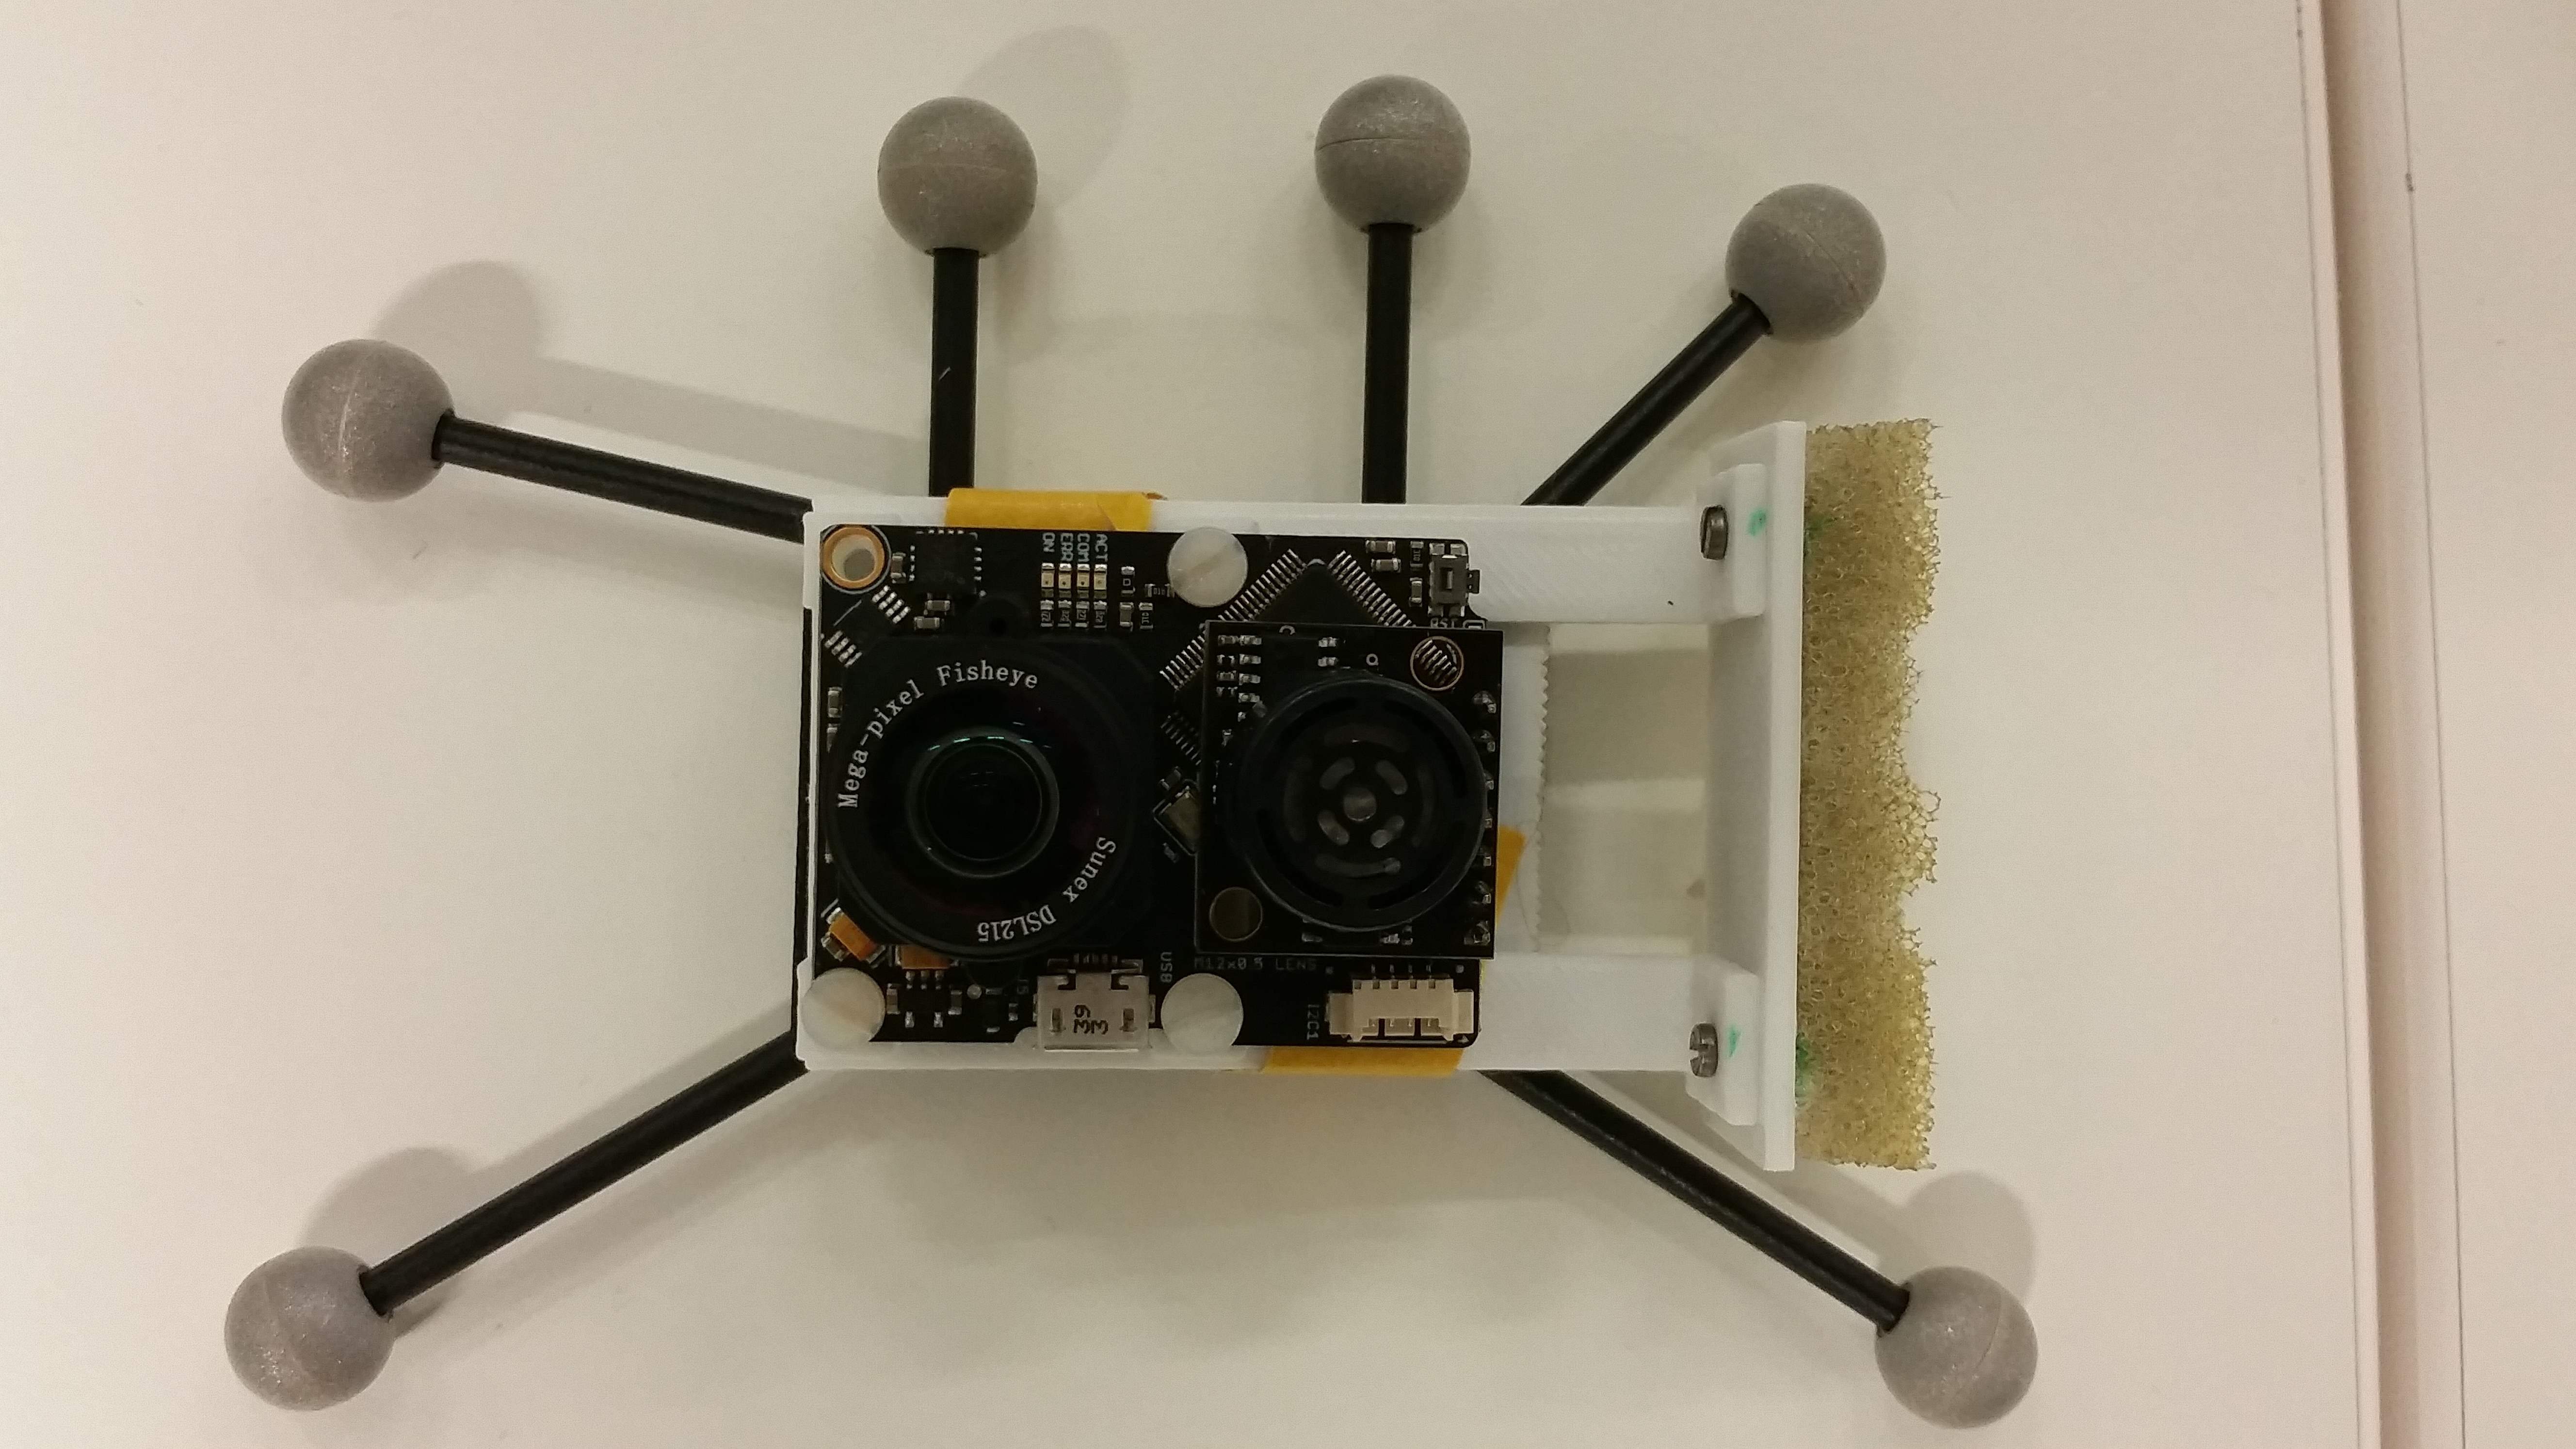
\includegraphics[width = 0.5\linewidth]{images/moCapFrame.jpg}
\caption{\textbf{Optic-flow sensor mounted on its motion capture frame} - The frame is equipped with 5 passive markers attached at known positions to obtain 3D position and orientation of the rigid body out of the 21 IR cameras.}
\end{figure}

Experiments were performed using an OptiTrack motion capture system which high precision allowed to estimate the ground truth measurements. The optic-flow sensor was mounted on a frame equipped with 5 markers (coated with a reflective material) attached at known positions to obtain the three-dimensional position and orientation of the rigid body (Fig.~\ref{fig:motionCapture}). The motion of the camera was recorded at 250Hz using a set of 21 IR cameras. The measured orientation are differentiated so as to obtain the angular rates of the rigid body, which are compared to the gyroscopes measurements for synchronization purposes (convolution).


Motion capture using passive markers requires the emission of IR lights that are sensed by the camera due to its small size. Due to the frequency at which these articial lights were emitted (250Hz), the ambiant illumination as seen by the camera (200Hz) typically changed every 150ms inducing an automatic calibration of the luminosity, which requires extra 5ms before new readings are sampled. Although this setup was kept due to time constraints, this issue could be avoided by switching of IR lights and using active markers (i.e. a set IR LEDs).

\subsection{Results}